\documentclass[12pt, border=3mm]{standalone}
\usepackage{tikz}
\usepackage{tkz-euclide}

\begin{document}
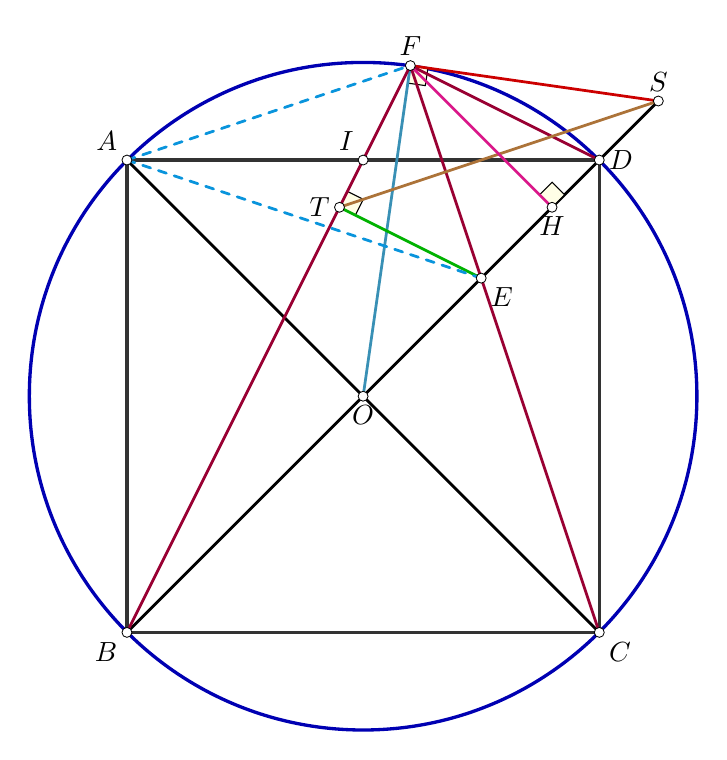
\begin{tikzpicture}[scale=1.5]
    % Define points
    \tkzDefPoint(0,0){O}
    \tkzDefPoint(-2,2){A}
    \tkzDefPoint(-2,-2){B}
    \tkzDefPoint(2,-2){C}
    \tkzDefPoint(2,2){D}
    \tkzDefPoint(1,1){E}
    \tkzDefPoint(0.4,2.8){F}
    \tkzDefPoint(2.5,2.5){S}
    \tkzDefPoint(1.6,1.6){H}
    \tkzDefPoint(-0.2,1.6){T}
    \tkzDefPoint(0,2){I} % Giao điểm AD và BF
    
    % Styling
    \tikzset{
        c_circle/.style={thick, color=blue!70!black, line width=1.2pt},
        c_square/.style={thick, color=black!80, line width=1.2pt},
        c_diag/.style={color=black, line width=1pt},
        c_cef/.style={color=orange!90!black, line width=1pt},
        c_of/.style={color=cyan!70!black, line width=1pt},
        c_tangent/.style={color=red!80!black, line width=1pt},
        c_bf/.style={color=purple!80!black, line width=1pt},
        c_st/.style={color=brown!90!black, line width=1pt},
        c_fh/.style={color=magenta!90!black, line width=1pt},
        c_et/.style={color=green!70!black, line width=1pt},
        c_sol/.style={color=cyan!80!blue, line width=1pt, dashed}
    }
    
    % Draw Circle and Square
    \tkzDrawCircle[c_circle](O,A)
    \tkzDrawPolygon[c_square](A,B,C,D)
    
    % Draw main diagonals
    \tkzDrawSegments[c_diag](A,C B,S)
    
    % Mark right angles
    \tkzMarkRightAngles[size=0.15, fill=yellow!10](O,F,S F,H,S E,T,F)
    
    % Draw problem lines
    \tkzDrawSegments[c_of](O,F)
    \tkzDrawSegments[c_tangent](F,S)
    \tkzDrawSegments[c_bf](B,F C,F F,D)
    \tkzDrawSegments[c_st](S,T)
    \tkzDrawSegments[c_fh](F,H)
    \tkzDrawSegments[c_et](E,T)
    
    % Draw solution auxiliary lines
    \tkzDrawSegments[c_sol](A,F A,E)
    
    % Mark points
    \foreach \p in {O,A,B,C,D,E,F,S,H,T,I} {
        \filldraw[fill=white, draw=black, line width=0.3pt] (\p) circle (1.2pt);
    }
    
    % Labels
    \tkzLabelPoint[above left](A){$A$}
    \tkzLabelPoint[below left](B){$B$}
    \tkzLabelPoint[below right](C){$C$}
    \tkzLabelPoint[right](D){$D$}
    \tkzLabelPoint[above](S){$S$}
    \tkzLabelPoint[below](O){$O$}
    \tkzLabelPoint[below right](E){$E$}
    \tkzLabelPoint[above](F){$F$}
    \tkzLabelPoint[below](H){$H$}
    \tkzLabelPoint[left](T){$T$}
    \tkzLabelPoint[above left](I){$I$}
\end{tikzpicture}
\end{document}
